\documentclass[11pt,a4paper]{article}

\usepackage[a4paper]{geometry}
\usepackage{fullpage}
\usepackage{fancyhdr}
\usepackage{lastpage}
\usepackage{mathtools}
\usepackage{gensymb}
\usepackage{fontspec}
\usepackage{color}
\usepackage{graphicx}
\usepackage{wrapfig}
\usepackage{tabularx}
\usepackage{hyperref}
\usepackage[french]{babel}
\usepackage{indentfirst}
\usepackage{multicol}
%\usepackage{float}
\usepackage{mdwlist}
\usepackage{bnf}
\usepackage{listliketab}
\usepackage[export]{adjustbox}
\usepackage{subfigure}

\usepackage{xcolor}
\usepackage{listings}
\renewcommand{\lstlistingname}{Extrait de code}
\lstset{basicstyle=\ttfamily,
  showstringspaces=false,
  commentstyle=\color{gray},
  keywordstyle=\color{blue}
}



\newcommand\vartitle{Implémentation d'un compilateur simplifié}
\newcommand\varauthor{Federico Pfeiffer}
\newcommand\vardate{\today}

\title{\vartitle}
\author{\varauthor}
\date{\vardate}

\pagestyle{fancyplain}
\lhead[\vartitle]{\vartitle}
\chead[]{}
\rhead[\varauthor]{\varauthor}
\lfoot[]{}
\cfoot[\thepage\ of \pageref{LastPage}]{\thepage\ of \pageref{LastPage}}
\rfoot[]{}

\renewcommand{\headrulewidth}{0.2mm}
\renewcommand{\footrulewidth}{0mm}

\setlength{\headsep}{40pt}

\setlength{\columnsep}{30pt}

\setlength{\parindent}{0mm}
\setlength{\parskip}{2mm}

\setcounter{secnumdepth}{3}
\setcounter{tocdepth}{2}


\hypersetup{
  hidelinks,
  pdfstartview={FitV},
  pdftitle={\vartitle},
  pdfauthor={\varauthor}
}

\begin{document}

  \begin{titlepage}
    \maketitle

    \thispagestyle{empty}

    \begin{abstract}
    Ce rapport décrit l'implémentation d'un compilateur du langage Hepial, défini les spécifications en annexe.
    \end{abstract}

%    \vspace{1cm}

    \tableofcontents

  \end{titlepage}

  \newpage

  \section{Présentation}
  
  \subsection{État général de l'implémentation}  
  
    \par Le compilateur a pu être implémenté selon le cahier des charges demandé: il analyse syntaxiquement un code source en créant un arbre abstrait et une table des symbole, puis recherche les erreurs sémantiques possibles au sein de l'arbre abstrait et la table des symboles. Si aucune erreur a été détectée, le compilateur produit un code source en jasmin, qui est ensuite compilé en byte code .class. 
    
     \par La notion de récursivité de fonctions, et de portée des variables ont également pu être implémentée. De même, des expressions complexes telles que celles-ci ont également pu être implémentées. \textit{if( a < b || 2*6+4 > 0)}. Enfin, des imbrications de boucles (telles que while et for) sont également possible. 
     
     \par Bien que les tableaux aient été ajoutés, ceux-ci n'ont été que très peu testés. Plusieurs dimensions sont en théories possibles, mais cela n'a pas été testé non plus. La gestion des tableaux a été définie de la sorte: array[5 .. 10] crée un tableau de 5 cases, dont l'index va de 0 à 5. 
     
     \par Enfin, l'expression \textit{inégal} s'écrit \textit{!=} au lieu de \textit{<>}. Par ailleurs, la déclaration de fonction au sein d'une fonction est interdite par soucis de simplicité.
     
  \subsection{Utilisation}
  
  \par L'utilisation du compilateur se fait de la manière suivante: 

  \begin{enumerate}
  \item Compilez le compilateur avec la commande \textit{make}. Cela va générer un dossier \textit{/bin/} contenant le byte code du compilateur. L'exécutable nommé \textit{hepiaCompile} sera généré dans le même dossier où se trouve le fichier \textit{make}. (Pas besoin de changer de dossier avec \textit{cd}).  
  \item Compilez ensuite le fichier hepial avec la commande \textit{bash hepiaCompile} suivit du nom du fichier Hepial à compiler. Cela va générer un dossier \textit{compiledBin} contenant le byteCode du programme Hepial, ainsi que ses sources en jasmin. L’exécutable du programme sera généré dans le même dossier où se trouve le fichier \textit{make}.
  \end{enumerate}
  
  \begin{lstlisting}[language=bash,caption={Utilisation du compilateur}]
    
    # compiler le compilateur
    $ make 
    
    # compiler le fichier hepial
    $ bash hepiaCompile <fileName>  # fileName = input.txt par défaut
    
    # lancer l exécutable compilé
    $ bash <programName>
  \end{lstlisting}

\newpage  
  
  \subsection{Vue d'ensemble}
  
  \par La compilation s'exécute dans cet ordre:
  \begin{enumerate}
    \item Génération de l'arbre abstrait, de la table des symboles pendant le parsing syntaxique de Cup. 
    \item Vérification sémantique dans l'arbre abstrait et dans la table des symboles. 
    \item Production du code: fichiers jasmin et fichier .class. 
  \end{enumerate}
  
  \par  Les diverses étapes de la compilation sont exécutées depuis le fichier \textit{HepialCompilateur.java}, à l'intérieur de la fonction \textit{main}.

%  \begin{figure}[h]
%   \centering
%    \vspace*{\fill}
%    \subfigure[Déroulement général]{\label{fig:a} 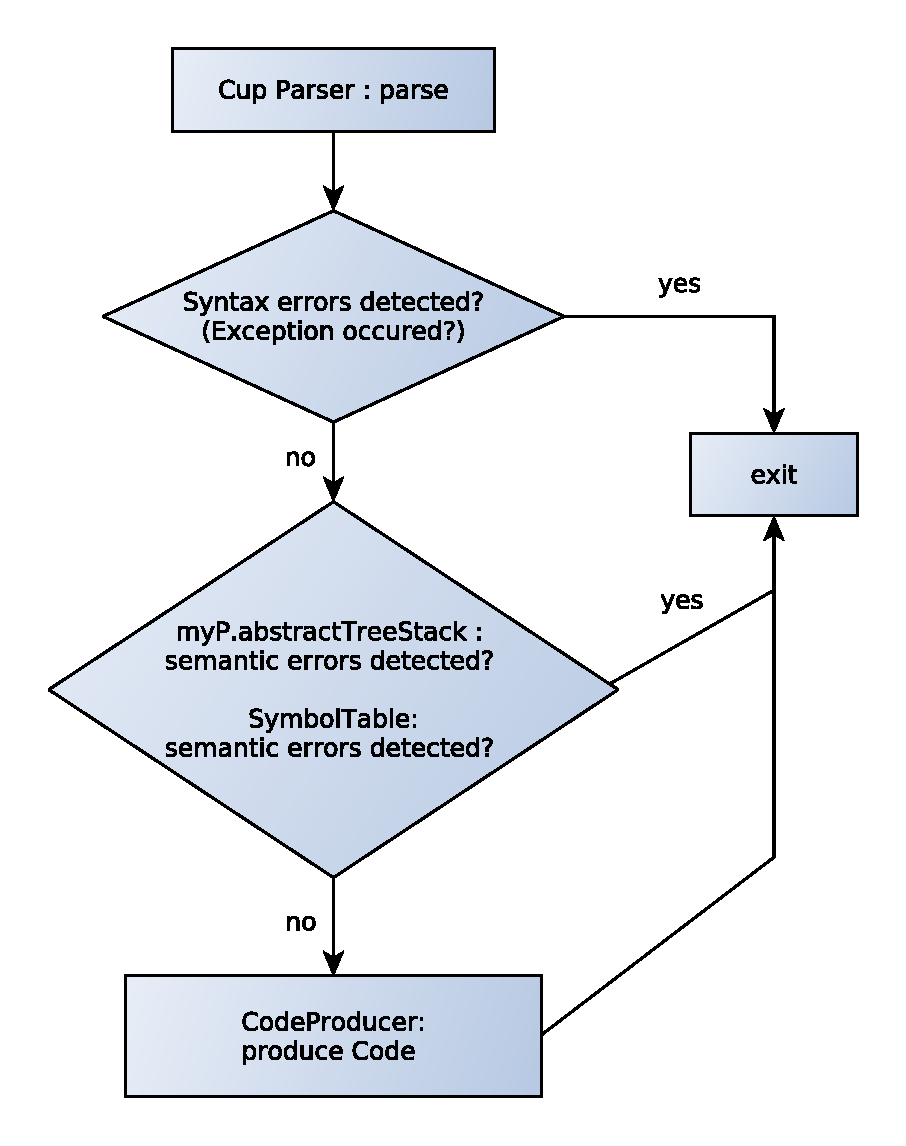
\includegraphics[width=70mm]{../ressources/mainProgramFlowChart.eps}}
%    \subfigure[Figure B]{\label{fig:a}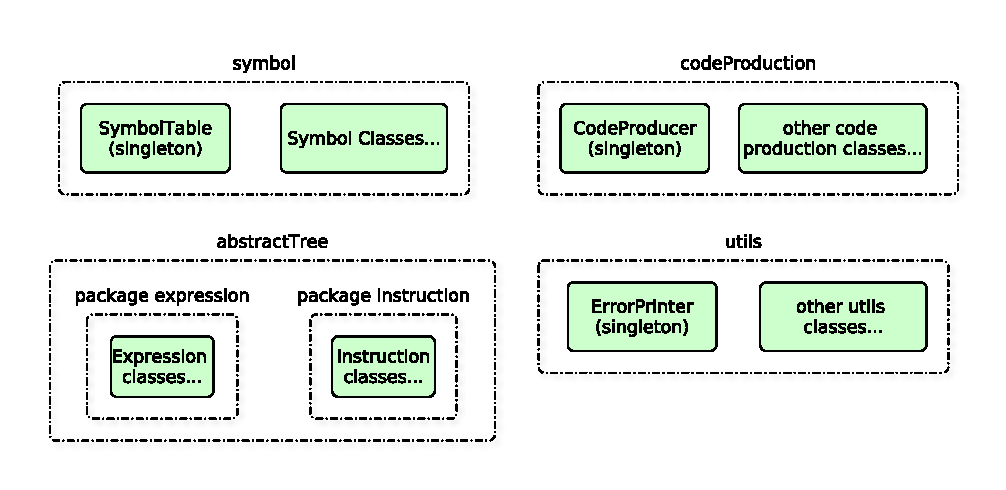
\includegraphics[width=80mm]{../ressources/packagesOverview.eps}}
%    \caption{Caption for this figure with two images}
%    \label{fig:image2}
%  \end{figure}   
  \begin{figure}[h]
    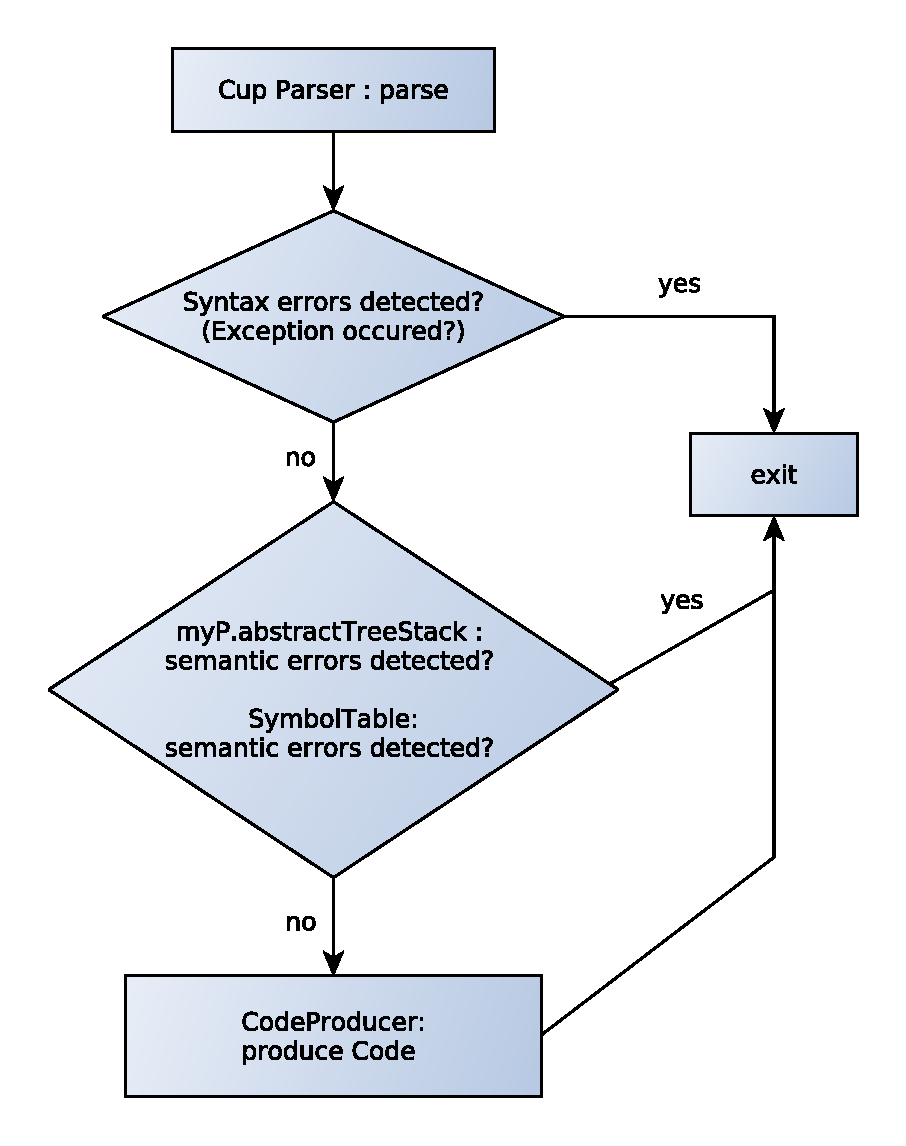
\includegraphics[width=.5\textwidth,center]{../ressources/mainProgramFlowChart.eps}
        \caption{Déroulement général du programme (fonction main())}
   \end{figure}

    \begin{figure}[h]
    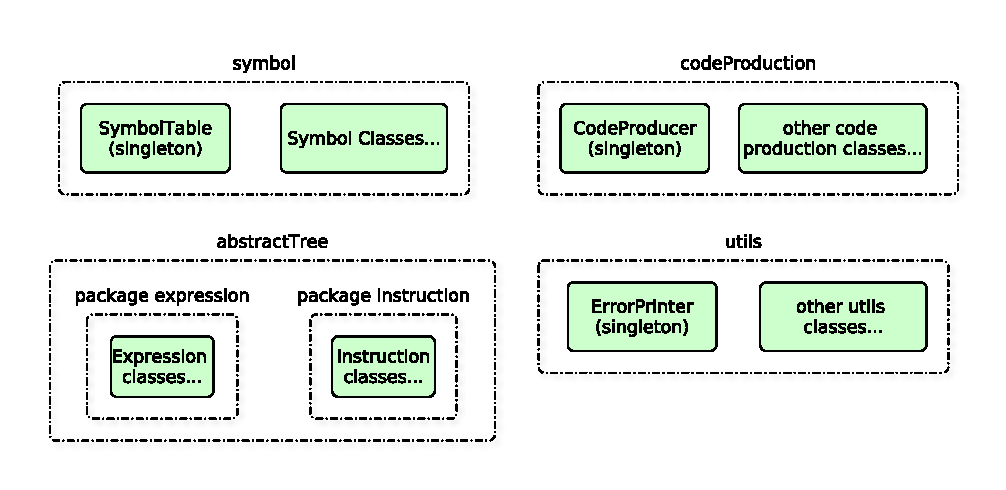
\includegraphics[width=.75\textwidth,center]{../ressources/packagesOverview.eps}
        \caption{Vue générale des packages et des principales classes}
   \end{figure}
   
   
   \section{Construction de l'arbre abstrait et table des symboles}
   
   \subsection{Arbre abstrait}
   
   \par L'arbre abstrait et la Table des Symboles sont générés pendant le parsing CUP, dans la première partie de la compilation. 
   
   \par Les expression et instructions héritent de la classe AsbtractTree. Les expressions et instructions détectées pendant le parsing CUP sont transmises de règle en règle à travers la pile de l'arbre abstrait, en empilant/dépilant les éléments de l'arbre abstrait. L'arbre abstrait est défini dans une des entêtes CUP.
   
   \begin{lstlisting}[caption={Déclaration de la pile de l'arbre abstrait}]
  init with {:
    abstractTreeStack = new Stack<AbstractTree>();
  :};
  \end{lstlisting}
  
  \par À la fin du parsing, on obtient un seul élément dans la pile d'arbre abstrait: un BlocInstruction contenant toutes les instructions du programme. Les instructions des fonctions se trouvent dans le symbol FunctionSymbol, ajouté dans la table des symboles. 
  
    \begin{figure}[h]
    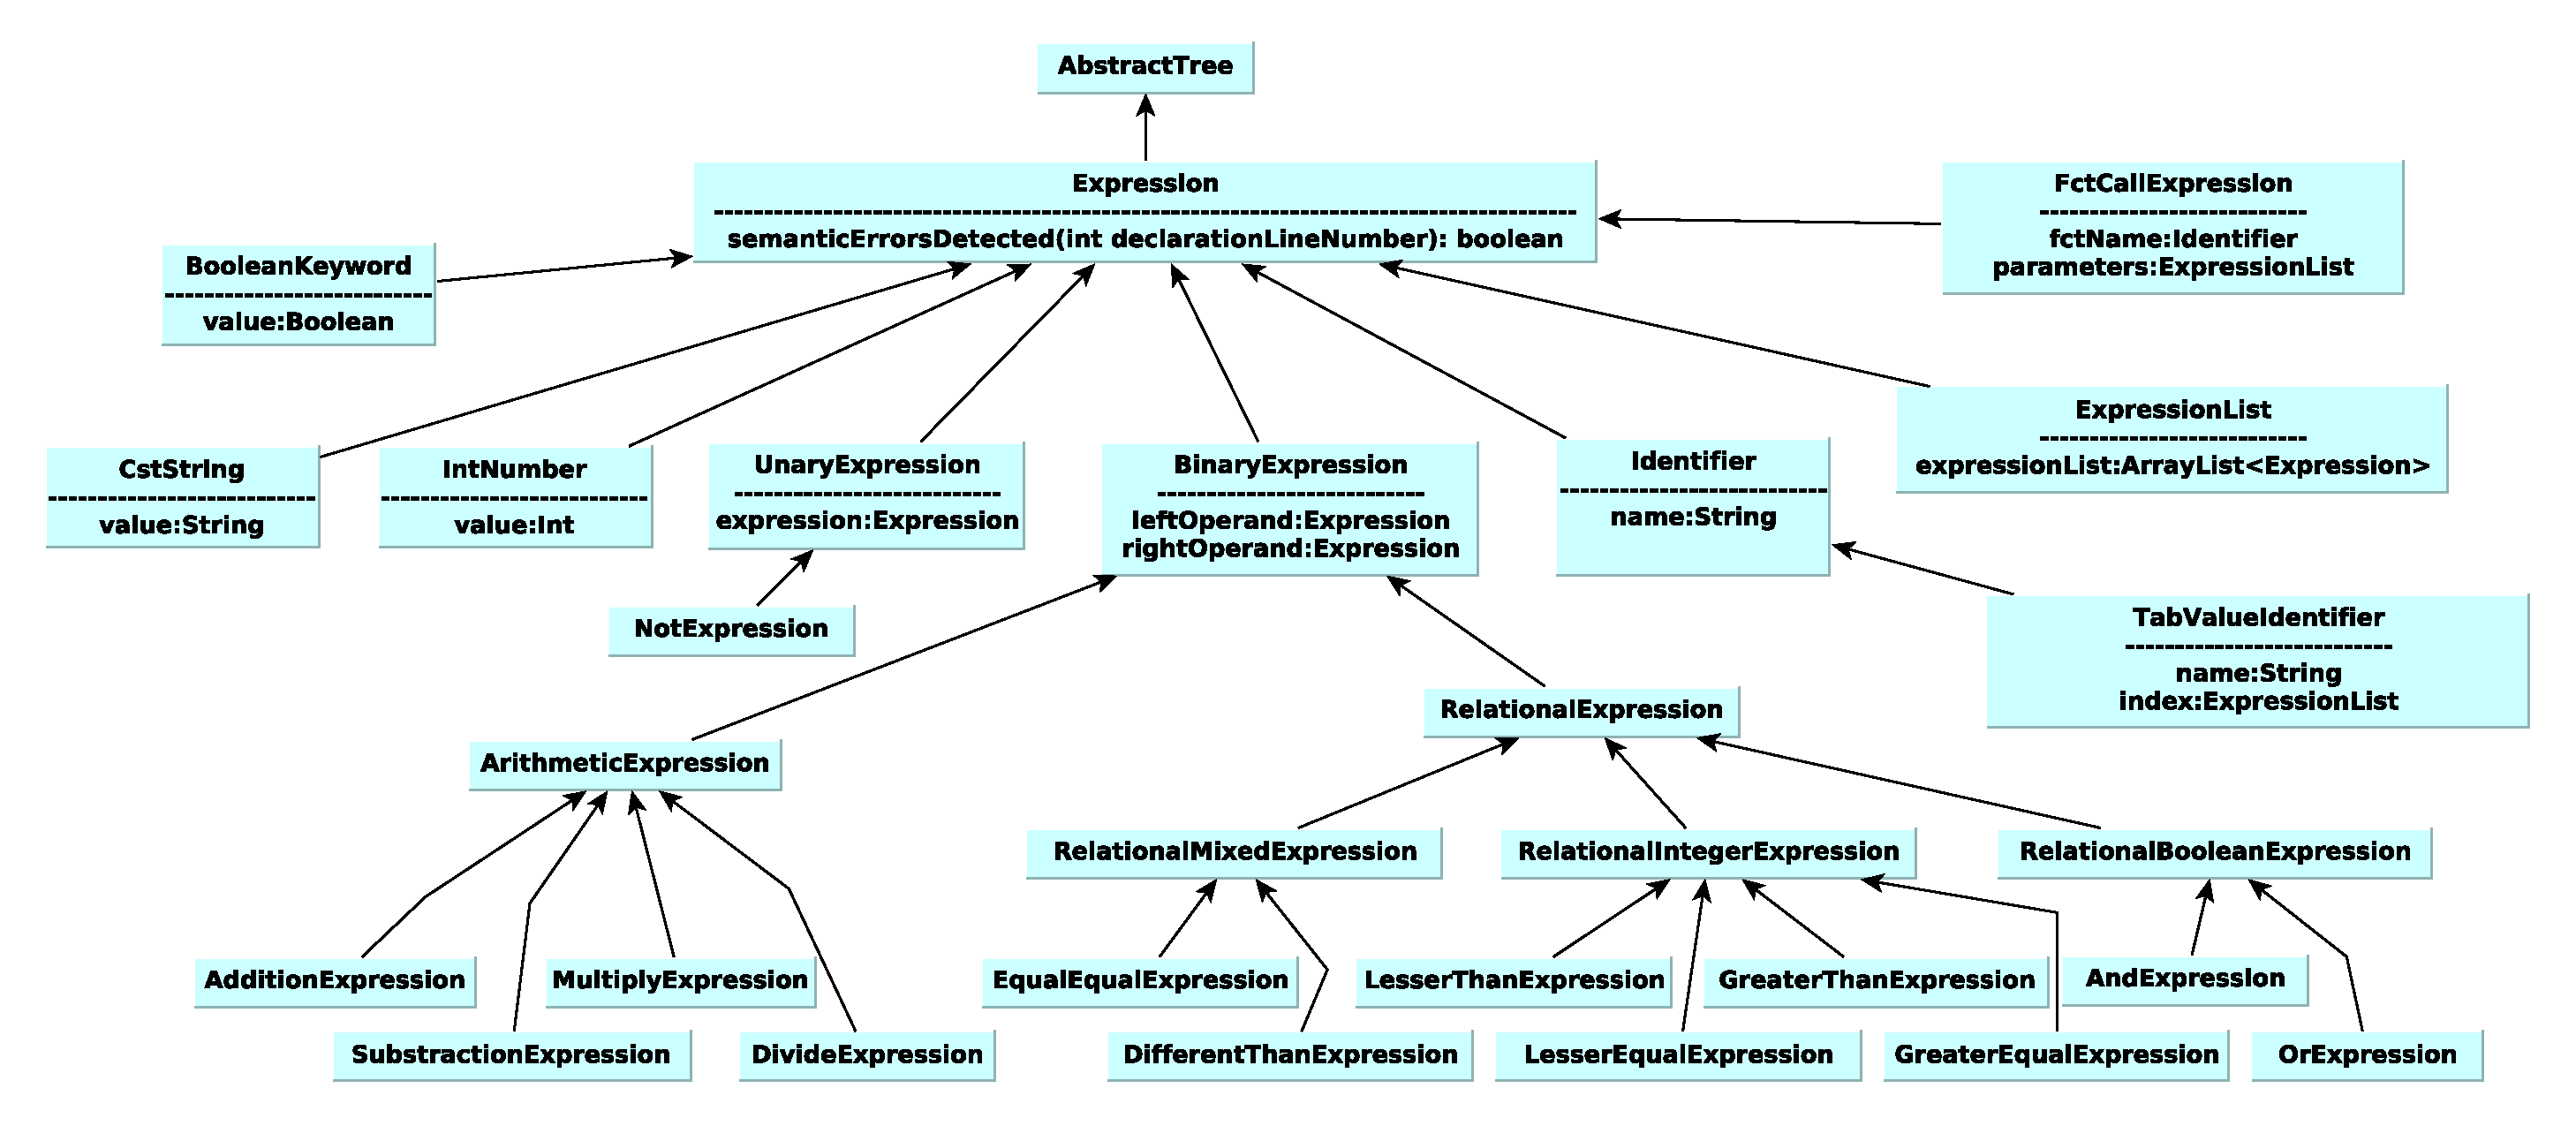
\includegraphics[width=1\textwidth,center]{../ressources/classesDExpressions.eps}
        \caption{Architecture des classes d'expressions}
   \end{figure}
   \newpage
    \begin{figure}[h]
    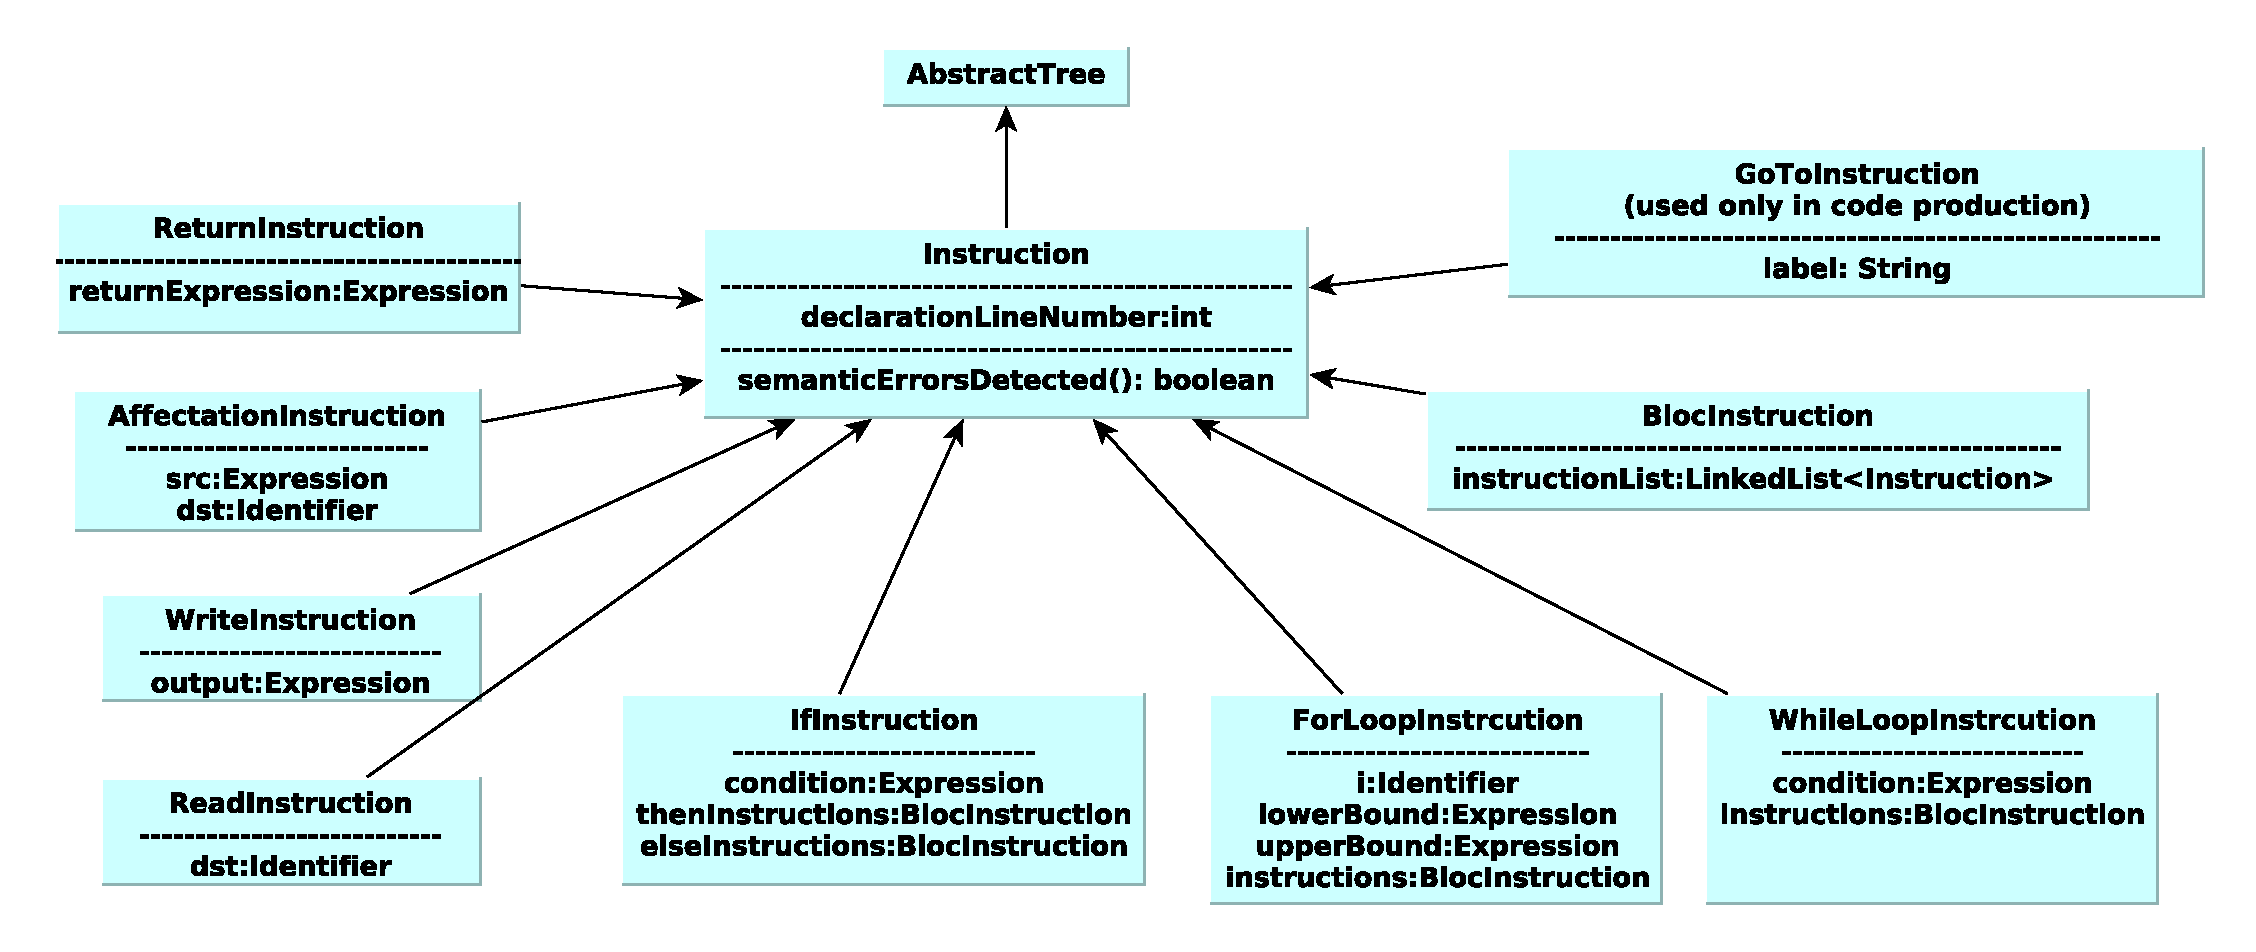
\includegraphics[width=1\textwidth,center]{../ressources/classesDInstructions.eps}
        \caption{Architecture des classes d'instructions}
   \end{figure}
  
  \subsection{Table des symboles}
  
  \par Les déclarations (telles que déclaration de fonction ou de variables) détectées pendant le parsing cup sont transmises de règles en règles à l'aide du RETURN de chaque règle. Elles sont transmises en tant que \textit{ArrayList<VarName, Symbol>}, ou plus précisément \textit{ArrayList<SimpleEntry<String, Symbol> >}. \\
  Ces éléments sont ensuite insérés dans la table des symboles par la règle adéquate. \\
  La table des symboles, de classe \textit{SymbolTable} est un singleton qui peut être accédée de manière statique à n'importe quel endroit du programme. 
  
   \begin{figure}[h]
    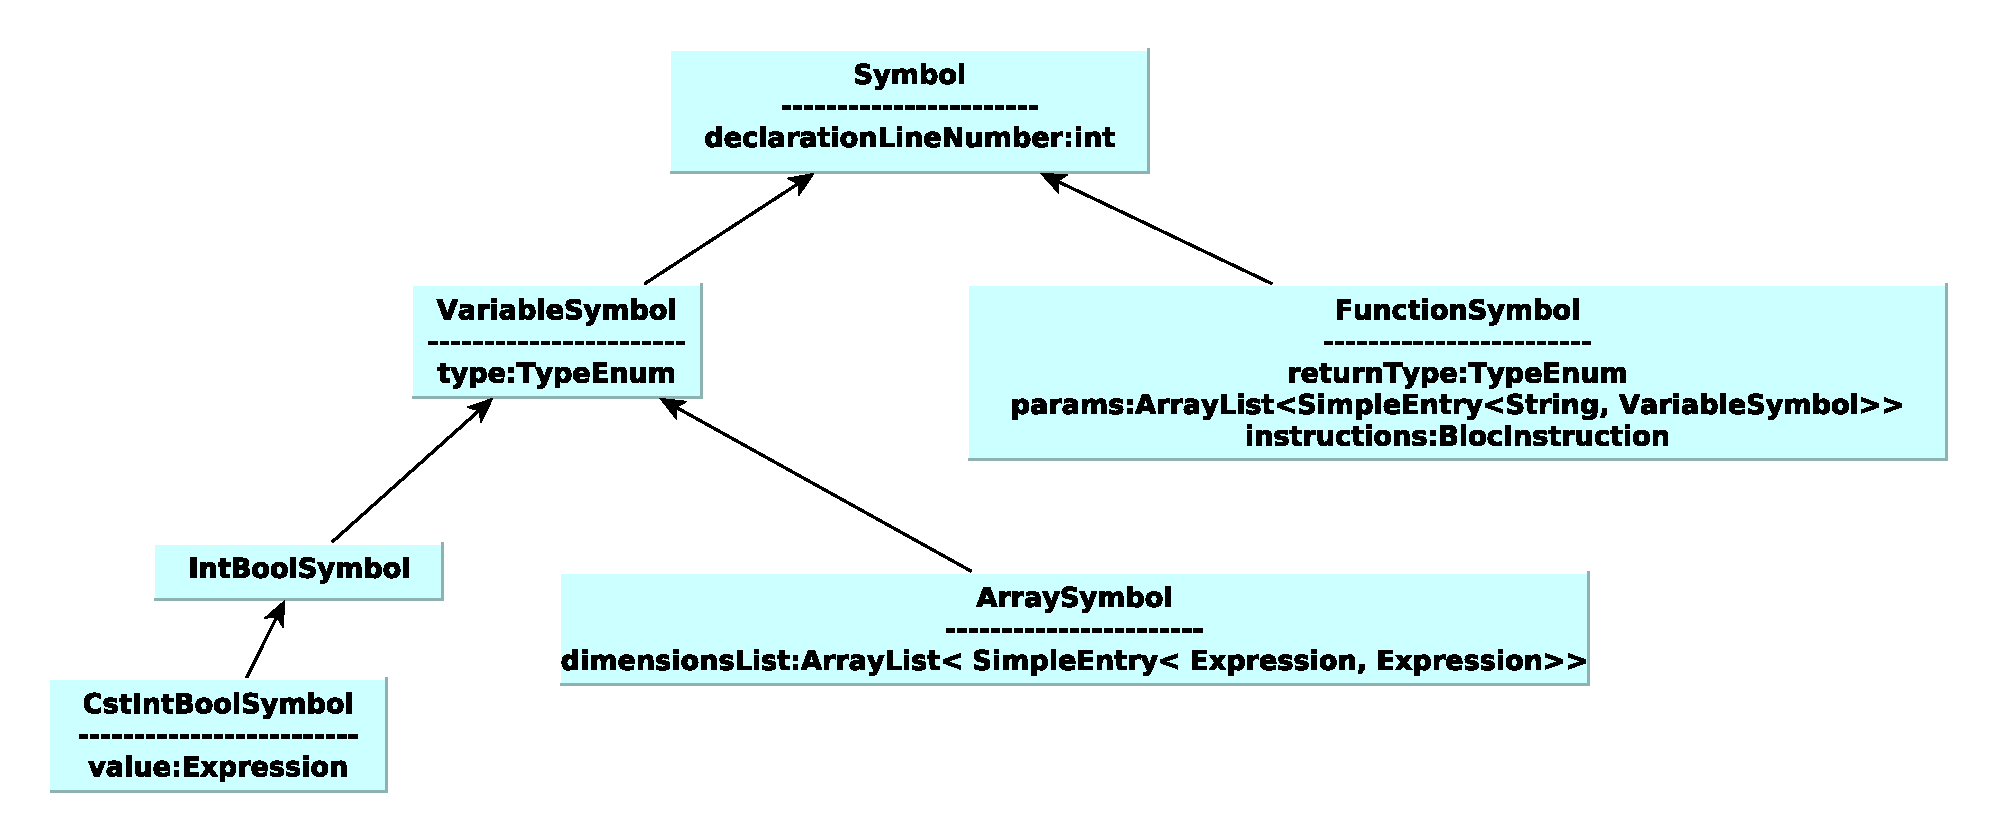
\includegraphics[width=1\textwidth,center]{../ressources/classesDesSymboles.eps}
        \caption{Architecture des classes de symboles}
   \end{figure}
   
   \subsection{Vérification syntaxique}
   
   \par La vérification syntaxique se fait par CUP directement. Si une erreur de syntaxe est détectée, une exception est levée et le compilateur affiche "parse error".   
   
   
  \section{Vérification sémantique}

  \subsection{Pattern utilisé}
  
  \par La vérification sémantique se fait une fois le parsing cup effectué. Nous nous retrouvons avec une tables des symboles complète, et une pile d'arbre abstrait contenant uniquement un bloc d'instructions \textit{(BlockInstruction)}. 
  
  \par A partir de là, le plus simple pour moi était d'utiliser le pattern \textit{Controller} défini dans les documents de cours. Si j'ai bien compris, il se rapproche du pattern \textit{Template method pattern} défini sur Wikipedia. Chaque classe de l'arbre abstrait comporte la méthode \textit{semanticErrorsDetected()}. Cette fonction vérifie si l'instance comporte des erreurs syntaxiques, et appelle la fonction  \textit{semanticErrorsDetected()} de tous les attributs de type arbre abstrait que l'instance contient. \\
  Elle renvoie faux si une erreur a été détectée soit au sein de l'instance, soit au sein d'un de ses attributs. 

  \par Par exemple, la fonction \textit{WhileLoopInstruction.semanticErrorsDetected()} va vérifier que son attribut \textit{WhileLoopInstruction.condition} est bien de type booléen. La fonction va ensuite appeler \textit{WhileLoopInstruction.condition.semanticErrorsDetected()} et \\ \textit{WhileLoopInstruction.instructions.semanticErrorsDetected()}. 
  
  \par Le même pattern est utilisé pour la vérification sémantique au sein des symboles. La table des symboles contient elle aussi une fonction \textit{semanticErrorsDetected()} afin de vérifier les erreurs sémantique au sein de tous les symboles déclarés. 
  
  \subsection{Processus}
  
  \par Une fois ces méthodes définies, la vérification sémantique dans tout l'arbre abstrait, et dans tous les symboles peut être effectuée facilement depuis la fonction main, une fois le parsing syntaxique effectué. 
  
    \begin{lstlisting}[language=java,caption={Processus de vérification syntaxique}]
   // check for semantic errors and print errors if any
   boolean errorsDetected = false;
   if(SymbolTable.getInstance().semanticErrorsDetected()){
     errorsDetected = true;
   }
   if(abstractTreeElement.semanticErrorsDetected()){
     errorsDetected = true;
   }

   if(errorsDetected){
     	ErrorPrinter.getInstance().printErrors();
      	System.exit(1);
   }
   \end{lstlisting}
   
  \newpage
  \subsection{Affichage des erreurs}
  
  \par L'instance \textit{ErrorPrinter}, un singleton, permet aux fonctions \textit{semanticErrorsDetected()} d'y logger les erreurs trouvées lors de la vérifiacation sémantique. Une fois la vérification sémantique terminée, on peut appeler la fonction \textit{ErrorPrinter.getInstance().printErrors()} pour afficher les erreurs une à une. Cela permet d'effectuer une vérification sémantique complète, tout en loguant des erreurs, sans avoir à stopper la vérification sémantique à chaque fois qu'une erreur est trouvée. 
  
  \section{Production du code}
  
  \par La production du code consiste en produire une représentation du programme en fichiers jasmin, pour être ensuite converti en byteCode java, executable par la JVM. 
  
  \subsection{Architecture de base d'un programme Hepial}
  
  \par Le code ayant pour finalité d'être décrite comme du byteCode java, il parait approprié d'illustrer l'architecture d'un programme Hepial en une représentation java. 
  
  \par Une première classe est créée, contenant la méthode \textit{static main()}. Cette classe est nommée avec le nom du programme définit dans l'entête du code Hepial . La méthode \textit{static main()} sert uniquement à lancer une deuxième instance, \textit{MainBlock}, contenant comme attributs les variables définies dans le bloc principal. Les instructions du bloc principal sont définis dans la fonction \textit{MainBlock.mainFunction()}.
  
    \begin{lstlisting}[language=java,caption={Architecture de base d'un programme Hepial}]
    public class HepialProgramName{
      public static void main (String[] arg){
        MainBlock mainBlock = new MainBlock();
        mainBlock.mainFunction();
      }
    }
    
   public class MainBlock{
      // variables defined in main block go here
   
      public void mainFunction(){
          // main instructions go here
      }
    }
   \end{lstlisting}  
   
  \par Lors de la production du code, les fichier jasmin et .class du programme sont créées dans un dossier \textit{compiledBin}. L'exécutable en tant que tel du programme Hepial est un fichier bash créé dans le dossier parent de \textit{compiledBin}. Il se présente sous cette forme: 
  
  \begin{lstlisting}[language=bash,caption={Exécutable programme Hepial}]
   #/bin/sh
   java -cp compiledBin HepialProgramName
   \end{lstlisting}    
  
  \par Cette architecture a été choisie pour répondre aux enjeux définis dans la prochaine section. 
  
  \subsection{Enjeux}
  
  \par Une première difficulté fut de trouver un moyen relativement simple de debugger les fichiers jasmin produits. L'utilisation des locales de la JVM ne permettaient pas de savoir quelle variable était réellement appelée. Appeler un attribut (une variable) par son nom se révéla beaucoup plus pratique pour debugger. Je me suis donc penché sur l'utilisation de classes java afin de représenter les variables déclarées, comme attributs d'une classe. 
  
  \par La notion de portée des variables entre les fonctions fut également un enjeu majeur. La possibilité de créer des variables locales à la fonction déclarée, tout en pouvant appeler des variables déclarées hors de cette fonction était un deuxième argument pour utiliser des classes java pour chaque Bloc: Une classe pour le bloc principal, et une classe par fonction est une solution viable que j'ai choisi pour répondre à la notion de portée des variables. \\
  Chaque fonction créée peut être représentée sous forme d'une classe, dont le constructeur est appelé avec \textit{MainBlock} comme référence. 
  
  \par Un dernier enjeu était la notion de récursivité: une fonction pouvant s'appeler elle même, il fallait trouver un moyen de garder la portée des variables intègre. 
  
  \par Par conséquent, j'ai choisi l'architecture suivante pour représenter les fonctions d'un programme Hepial.  
  
  \subsection{Architecture d'une fonction}
  
  \par La représentation d'une fonction en jasmin/byteCode est la même que la représentation du \textit{MainBlock}, à la différence que le constructeur de la fonction a comme paramètre la référence au \textit{MainBlock} afin d'avoir accès aux variables de celui-ci. 
  
  \par Dans la classe fonction, des attributs supplémentaires sont ajoutés aux variables déclarées dans la fonction: les paramètres de la fonction elle même. 
  
  \par Afin d'illustrer ceci, prenons ce code Hepial de la figure suivante comme exemple. On crée une variable globale égale à 1. On définit une fonction prenant en paramètre un entier. Cette fonction a une variable locale. La fonction prends la valeur entré en paramètre, fait la somme entre celle-ci et la variable globale, puis affecte le résultat dans sa variable locale. Elle retourne ensuite la valeur de sa variable locale. 
  \newpage
    \begin{lstlisting}[caption={Architecture d'une fonction et de son appel}]
   programme hepialProgramName

   constante entier globale = 1;
   entier resultat;
   entier maFct(entier param1)
      entier locale;
      debutfonc
         locale = param1 + globale;
         retourne locale;
      finfonc
   debutprg
      resultat = maFct(2);
   finprg
   \end{lstlisting} 
   
   \par La version java du programme Hepial aura donc cette forme: 
   
    \begin{lstlisting}[language=java,caption={Architecture de base d'un programme Hepial}]
    public class MainBlock{
      public int globale;
      public int resultat;
   
      public void mainFunction(){
          MaFct maFct = new MaFct(this);
          resultat = maFct.mainFunction(2);
      }
    }
    
    public class MaFct{
      MainBlock mainBlock;
      public int locale;
      
      MaFct(MainBlock mainBlock){
         this.mainBlock = mainBlock;
      }
      
      int mainFunction(int param1){
          locale = this.mainBlock.globale + param1;
      }
    }
   \end{lstlisting}    
  
  
  
  \subsection{Principales instances de la production du code} 
  
  \subsubsection{CodeProducer}
  
  \par La production du code est appelée depuis la fonction main du compilateur, à l'aide de l'appel suivant: \textit{CodeProducer.getInstance().produceProgram()}. Cette fonction peut être représentée selon le schéma ci-dessous: 
  
  \begin{figure}[h]
    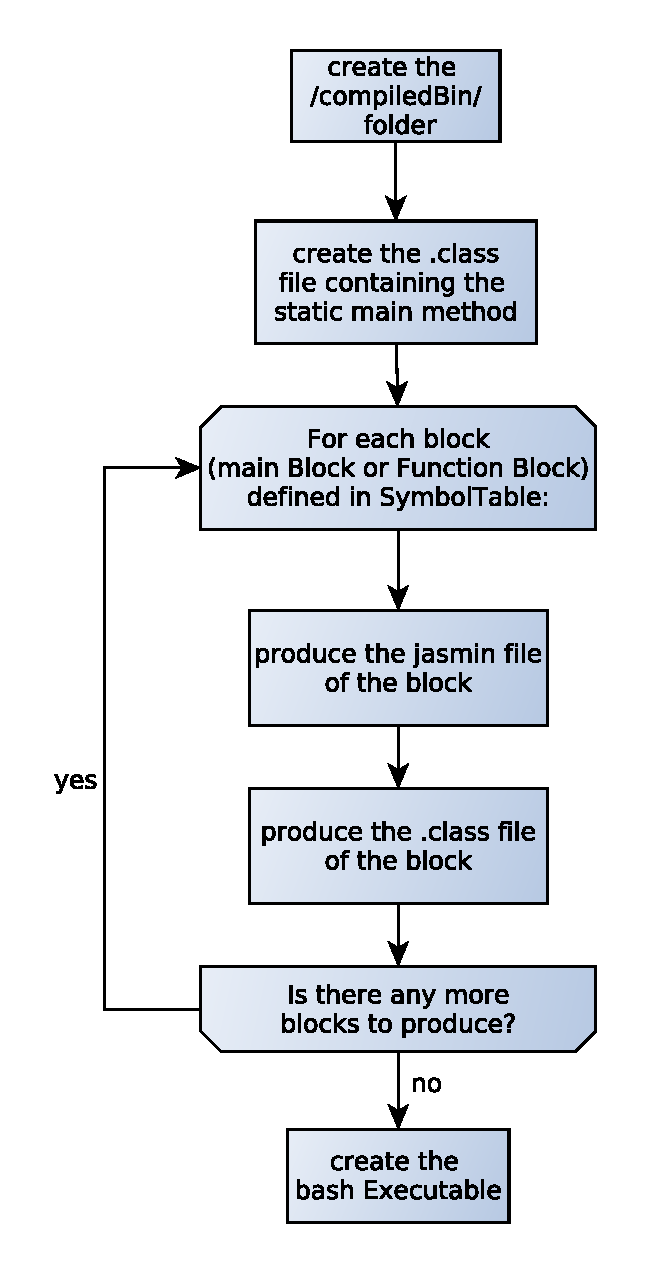
\includegraphics[width=0.4\textwidth,center]{../ressources/CodeProductionOverview.eps}
    \caption{Vue générale de la production de code}
  \end{figure}
  
  \subsubsection{Block}  
  
  \par Afin de créer les fichiers jasmin, \textit{CodeProducer} s'aide de la classe \textit{Block}. Cette dernière contient l'API nécessaire pour créer un fichier jasmin représentant chaque bloc du programme Hepial: à savoir le bloc principal, et les blocs représentant les fonctions déclarées. 
  
  \par Le schéma suivant illustre la manière dont la classe \textit{CodeProducer} crée les fichiers jasmin: 
  
  \newpage
    \begin{figure}[h]
    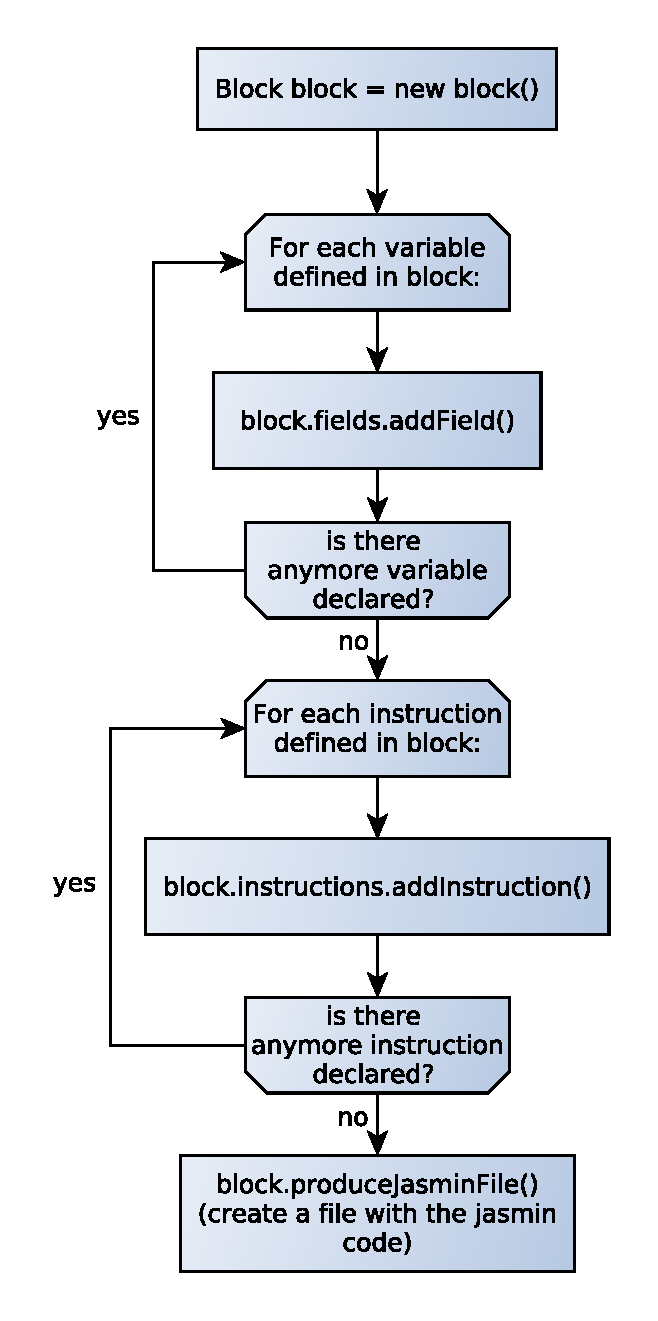
\includegraphics[width=0.4\textwidth,center]{../ressources/jasminFileProducionOverview.eps}
    \caption{Schéma général d'une production de code jasmin}
  \end{figure}
  
  \par Pour produire le code jasmin, la classe \textit{Block} a comme attributs des classes spécialisées dans la "vraie" production du code jasmin: à savoir produire un  texte jasmin en fonction de leur spécialité. Les attributs en question de la classe \textit{Block} sont les suivants: 
  
  \begin{itemize}
    \item constructor: de type ConstructorProducer
    \item localFiels: de type Fileds
    \item instructions : de type FunctionInstructions
  \end{itemize}
  
  \subsubsection{Block}
  
  \section{Exemples de compilation / exécution}
  
  \section{Améliorations possibles}
   
\end{document}
